\documentclass[a4paper,twoside,12pt]{article}
%\usepackage [reqno] {amsmath}
\usepackage{amsfonts,amstext}
\usepackage{amsmath}
\usepackage{ngerman}
\usepackage{fullpage}
\usepackage{xspace}
\usepackage{graphicx}
\usepackage{tikz}
\usetikzlibrary{trees}


\newcounter{AUFGNR}
\setcounter{AUFGNR}{1}
\newcommand{\AUFGABE}[2]{\vspace{0.3cm}\item[Aufgabe \arabic{AUFGNR}]\stepcounter{AUFGNR} #1\hfill\emph{#2}}


\newcommand{\floor}[1]{\left\lfloor{#1}\right\rfloor}
\newcommand{\ceil}[1]{\left\lceil{#1}\right\rceil}
\newcommand{\half}[1]{\frac{#1}{2}}
\newcommand{\N}{\mathbb{N}}

\renewcommand{\labelenumi}{(\alph{enumi})}


\begin{document}
\pagestyle{empty}
\hrule\medskip
\rule{0ex}{0ex}\\[-1ex]
Probeklausur zur Vorlesung

\smallskip
\noindent
\large
\textbf{Algorithmen und Datenstrukturen}\hfill SoSe 2025 \\[0.5ex]
\normalsize
Wolfgang Mulzer

\medskip\hrule

\smallskip
\noindent
Bearbeitungszeit: mindestens 90 Minuten

\vskip 0.5cm

\begin{description}

\AUFGABE{Datenstrukturen}{4+3+3 Punkte}

Sei $U$ eine total geordnete Menge. Wir wollen
Teilmengen $S \subseteq U$ speichern, so dass folgende Operationen
m\"oglich sind:
\begin{itemize}
  \item \texttt{insert}(x): Füge $x$ zu $S$ hinzu.
  \item \texttt{deleteMin}(): Voraussetzung: $S$ ist nicht leer. Das kleinste
	  Element aus $S$ soll gelöscht werden.
  \item \texttt{deleteMax}(): Voraussetzung: $S$ ist nicht leer.
	  Das größte Element aus $S$ soll gelöscht werden.
\end{itemize}
Sie dürfen annehmen, dass wir  zwei Elemente aus $U$ in 
konstanter Zeit vergleichen können. Für jede der folgenden drei
Datenstrukturen, beschreiben Sie jeweils kurz, wie man die 
Operationen \texttt{insert} und \texttt{deleteMax} 
möglichst effizient implementieren kann, und geben Sie möglichst
gute asymptotische obere Schranken für die Laufzeit.
Erklären Sie gegebenenfalls, welche zusätzlichen Annahmen nötig sind.

\begin{enumerate}
  \item AVL-Baum;
  \item Hashtabelle mit linearem Sondieren; 
  \item unkomprimierter Trie. 
\end{enumerate}

\newpage
\subsection*{Lösung Aufgabe 1:}
\paragraph{Gesucht:}
\begin{itemize}
	\item Operationen insert und delteMax
	\item obere Schranke der Laufzeit (Worst-case O-Notation)
	\item Vergleiche passieren in Konstanter Zeit also $O(1)$
\end{itemize}


\subsubsection*{AVL-Baum:}
\paragraph{insert(k):}
\begin{enumerate}
	\item Suche nach dem Schlüssel $k$ im Baum
	\begin{itemize}
		\item Beginne bei der Wurzel
		\item Vergleiche k mit n.k
		\begin{itemize}
			\item k $==$ n.k: Wert gefunden
			\item k $<$ n.k: gehe in den linken Teilbaum
			\item k $>$ n.k: gehe in den rechten Teilbaum
		\end{itemize}
		\item Falls $NULL$ erreicht: $k$ nicht vorhanden
		\item return die Position von $NULL$ oder $k$
	\end{itemize}
	\item Einfügen als neues Blatt oder Updaten von dem Vorhanden Wert an stelle $k$
	\begin{itemize}
		\item beim Updaten passiert nichts weiter mit der AVL-Eigenschaft, da sich keine Höhen ändern $\rightarrow$ wir sind fertig
	\end{itemize}
	\item Wenn wir ein neues Blatt einfügen $\rightarrow$ überprüfe den Pfad vom neuen Blatt bis zur Wurzel den Balance-factor der Knoten 
	\begin{itemize}
		\item BF = $|\text{Höhe des rechten Teilbaums}| - |\text{Höhe des linken Teilbaums}|$
		\item Wenn der BF $> 1$ müssen wir eine Rotation ausführen um den BF wieder herzustellen 
		\item mögliche Rotationen: links, rechts, linksrechts, rechtslinksrotation
		\begin{itemize}
			\item Baumstruktur links-links $\rightarrow$ R-Rotation
			\item Baumstruktur rechts-rechts $\rightarrow$ L-Rotation
			\item Baumstruktur links-rechts $\rightarrow$ LR-Rotation
			\item Baumstruktur rechts-links $\rightarrow$ RL-Rotation
		\end{itemize}
	\end{itemize}
\end{enumerate}

\paragraph{deleteMax():}
\begin{itemize}
	\item Von der Wurzel ausgehen verfolge den rechten Teilbaumpfad, bis zum ende, dort befindet sich in einem Binary Search Tree das größte Element(AVL-Baum ist eine Binary Search Tree)
	\item Lösche das Element
	\item Analog wie bei \texttt{insert(k)} den BF überprüfen und ggf. Rotationen ausführen
\end{itemize}

\paragraph{Laufzeit:} im Worst-case Fall
\begin{itemize}
	\item Suche(k) - O(log n) - Da der ein AVL-Baum selbstbalancierend ist, kann er nicht so stark degenerieren, das wir ein links- oder rechtsgerichteten Baum erhalten
	\item insert(k) - O(log n) - wie beim Suchen ähnliche Struktur
	\item deleteMax() - $O(\log n)$ - Suchen $O(\log n)$ Löschen $O(1)$
	\item Rebalancieren - $O(\log n)$ 
\end{itemize}


\subsubsection*{Hashtabelle mit linearem Sondieren:}
\paragraph{insert(k):}
\begin{itemize}
	\item Berechne den Hashwert von h(k) und gehen an die Stelle im Array
	\item Wenn die Stelle $NULL$ ist einfügen von (k,v)
	\item Wenn die Stelle belegt ist gehe im Array weiter bis \texttt{NULL} gefunden wird
	\begin{itemize}
		\item Dabei Speichern wir die erste Position von \texttt{DELETED}
	\end{itemize}
	\item Am ende schauen wir ob wir eine \texttt{DELETED} position haben, wenn ja fürgen wir k dort ein, wenn nicht am ende wo wir \texttt{NULL} vorgefunden haben
\end{itemize}

\paragraph{deleteMax():} Hashtabellen gehören zu Dictionaries und die sind Ungeordnet, deshalb ist es uneffizient den Maximalwert des gesamten Arrays rauszufinden, wir müssten alle Entries durchgehen und Vergleichen was auf eine Laufzeigt von $O(\text{größe der Tabelle})$ hinauslaufen würde

\paragraph{Laufzeit:}
\begin{itemize}
	\item Suchen - Worst-case $O(\text{länge des Arrays})$, da wir bei linearem Sondieren, wenn ein Kollision auftritt den Eintrag immer weiterschieben, bis wir eine leere Position finden. Wenn das Array sehr voll ist kann es vorkommen das wir einmal das gesamte Array durchlaufen müssen.
	\item insert(k) - $O(n)$ Laufzeit hängt wie beim Suchen vom Füllgrad ab
	\item deleteMax() - siehe erklärung bei \texttt{deleteMax()}
\end{itemize}

\subsubsection*{unkomprimierter Trie:}
\paragraph{insert(k):}
\begin{itemize}
	\item Für jedes Zeichen $c$ im Schlüssel $s$
	\begin{itemize}
		\item Prüfe: gibt es eine ausgehende Kante für Symbol c?
		\begin{itemize}
			\item Wenn ja: Folge der Kante zum nächsten Knoten
			\item Wenn nein:
			\begin{itemize}
				\item Erstelle einen neuen Knoten
				\item Füge eine Kante mit Symbol $c$ hinzu, die zum neuen Knoten führt.
			\end{itemize}
		\end{itemize}
	\end{itemize}
	\item Nach dem letzten Zeichen:
	\begin{itemize}
		\item Markiere den Knoten als \texttt{Ende eines Schlüssels} mit z.B.: $\$$
	\end{itemize}
\end{itemize}

\paragraph{deleteMax():}
\begin{itemize}
	\item Vom Wurzelknoten aus:
	\begin{itemize}
		\item Folge immer der größten möglichen ausgehenden Kante, also das höchste Zeichen
		\item solange wie möglich nach rechts unten gehen
	\end{itemize}
	\item Sobald man bei einem Ende-Knoten landet z.B.: bei $\$$ $\rightarrow$ ist dies der größte gespeicherte Schlüssel
	\item Diesen löschen wir dann:
	\begin{itemize}
		\item Entferne den Ende-Marker
		\item Fall der Knoten von keinen anderen Schlüssel mehr benutzt wird, löschen wir den Knoten
	\end{itemize}
\end{itemize}

\paragraph{Laufzeit:}
\begin{itemize}
	\item insert(k): $O(|s| \cdot |\Sigma|)$
	\item deleteMax(): $O(|s_{max}| \cdot |\Sigma|)$
\end{itemize}

\newpage
\AUFGABE{Hashing}{1+5+4 Punkte}

\begin{enumerate}
\item Nennen Sie zusätzlich zu Hashing mit Verkettung noch zwei
  weitere Möglichkeiten der Kollisionsbehandlung in einer Hashtabelle.
\item
    Fügen Sie nacheinander die Schlüssel 5, 28, 19, 15, 20, 33, 12, 17, 10
    in eine Hashtabelle der Größe 9 ein. Die Hashfunktion sei
    $h(k) = k \bmod 9$. Die Konflikte werden mit linearem Sondieren
		gelöst. Verwenden Sie dafür das Schema auf der nächsten Seite.
\item
Beschreiben Sie einen Weg, wie man Kuckucks-Hashing mit \emph{drei}
Hashfunktionen implementieren kann. Geben Sie Pseudocode für
die Einfüge-Operation.
\end{enumerate}

\newpage
\subsection*{Lösung Aufgabe 2:}
\subsubsection*{a:}
\begin{enumerate}
	\item Hashing with linear probing
	\item Cuckoo Hashing
\end{enumerate}

\subsubsection*{b:}
Ich füge hier einfach das endergebnis ein:
\begin{center}
\begin{tabular}{|c|c|c|c|c|c|c|c|c|}
	\hline
	0 & 1 & 2 & 3 & 4 & 5 & 6 & 7 & 8 \\
	\hline
	10 & 28 & 19 & 20 & 12 & 5 & 15 & 33 & 17 \\
	\hline
\end{tabular}

\end{center}

\subsubsection*{c:}

\begin{verbatim}
put(k, v):
	// if k is present, we simply update the value
	if (T[h1(k)].k == k)
		T[h1(k)].v <- v
		return
	if (T[h2(k)].k == k)
		T[h2(k)].v <- v
		return
	if (T[h3(k)].k == k)
		T[h3(k)].v <- v
		return
	// if not, we must insert (k, v)
	// if the table is already full, we cannot insert $k$
	if (|S| == N)
		throw TableFullException
	// we try to insert the entry at the first position
	pos <- h1(k)
	for i := 1 to N do
		// if the position is empty, we insert the entry
		// and are done
		if (T[pos] == NULL)
			T[pos] <- (k,v)
			return
		// otherwise, we exchange the current entry and
		// determine the second possible position
		(k,v) <-> T[pos]
		if (pos == h1(k))
			pos <- h2(k)
		else if (pos == h2(k))
			pos <- h3(k)
		else
			pos <- h1(k)
	// if the insertion does not succeed, we need to rebuild the table
	Choose new hash functions and rebuild the table
	put(k,v)
\end{verbatim}


\newpage
\AUFGABE{Vermischtes}{2+2+2+2+2 Punkte}

\begin{enumerate}
  \item  
     Nennen Sie zwei Eigenschaften und zwei mögliche  Anwendungen von kryptographischen Hashfunktionen.
  \item Wahr oder falsch: Der Algorithmus von Dijkstra funktioniert auch in Graphen mit
	  negativen Kantengewichten. Begründen Sie Ihre Antwort.
  \item Zeichnen Sie einen komprimierten
    Trie für die Wörter KLAUSUR, KLASSE, KLEEBLATT, KLEISTER.
    \item
	    Wahr oder falsch: Ein binärer Baum der Höhe $h$ besitzt immer mindestens
		$2^h$ Knoten. Begründen Sie Ihre Antwort. (Zur Erinnerung: 
		Die \emph{Höhe} bezeichnet die maximale Anzahl von Kanten von der
		Wurzel des Baumes bis zu einem Blatt.)
	\item Nennen Sie einen Vorteil und einen Nachteil von $(a, b)$-Bäumen gegenüber
		AVL-Bäumen.
\end{enumerate}

\newpage
\subsection*{Lösung Aufgabe 3:}
\subsubsection*{Teilaufgabe (a):}
\paragraph{Eigenschaften:}
\begin{itemize}
	\item Schnell berechenbar für beliebige Eingaben
	\item Kollisions resistent: Es ist praktisch unmöglich, zwei vverschiedene Eingaben zu finden, die denselben Hashwert haben
\end{itemize}

\paragraph{Anwendungen:}
\begin{itemize}
	\item Passwort-Hashing - man Speichert beim eingeben des Passworts nicht das Passwort in Klartext, sondern nur den Hash-Wert
	\item Hash-Referenzen und Blockchain - Durch das Speichern von Hashreferenzen in Objekten kann man Manipulation am Objekt sehr leicht erkennen, da die Hash-Werte nicht mehr übereinstimmen
\end{itemize}

\subsubsection*{Teilaufgabe (b):}
\paragraph{Antwort:} Falsch
\paragraph{Begründung:} Dijkstra funktioniert nicht in Graphen mit negativen Kantengewichten, weil er Algorithmus einmal gefundene minimale Distanzen als endgültig markiert. Sollten doch negative Kanten existieren, könnten spätere kürzere Wege existieren, die Dijkstra nicht mehr berücksichtigt.

\subsubsection*{Teilaufgabe (c):}
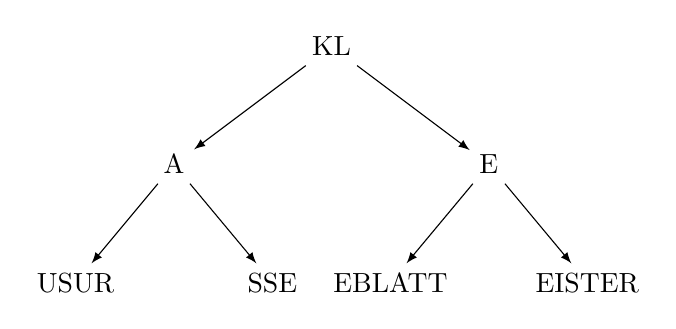
\begin{tikzpicture}[
	level 1/.style={sibling distance=40mm},
	level 2/.style={sibling distance=25mm},
	level 3/.style={sibling distance=15mm},
	edge from parent/.style={draw, -latex}
	]
	
	\node {KL}
	child {node {A}
		child {node {USUR}}
		child {node {SSE}}
	}
	child {node {E}
		child {node {EBLATT}}
		child {node {EISTER}}
	};
	
\end{tikzpicture}

\subsubsection*{Teilaufgabe (d):}
\paragraph{Antwort:} Falsch
\paragraph{Begründung:} Ein binärer Baum der Höhe $h$ kann im Worst-case nur $h+1$ Knoten besitzen - z.B.: wenn wir einen degenerierten Baum in Kettenform gegeben haben, dort hätte jeder Knoten nur genau ein Nachfolger. Das Minimum wäre also linear und nicht exponentiell.

\subsubsection*{Teilaufgabe (e):}
\paragraph{Vorteil:} $(a,b)$-Bäume sind besser für externe Speicher, wie Festplatten, geeignet, weil sie weniger Knotenbesuche pro Suche benötigen -dadruch werden Speicherzugriffe reduziert.
\paragraph{Nachteil:} Suchen und Updaten innerhalb eines Knotens, der viele Einträge(Schlüssel) enthält, sind aufwändiger als bei AVL-Bäumen. Da bei AVL-Bäumen jeder Knoten nur ein Schlüssel enthält. $(a,b)$-Bäume haben zusätzlich einen höheren, dafür aber konstanteren Speicherbedarf.

\newpage
\AUFGABE{Graphen}{6+4 Punkte}

\begin{enumerate}
  \item Führen Sie im folgenden ungewichteten Graphen eine Breitensuche durch, um die kürzesten
	 Wege  ausgehend vom Knoten $s$ zu ermitteln. 

		Verwenden Sie dafür das Schema auf der nächsten Seite. Der Pseudocode für BFS ist 
		wie folgt:
		\begin{verbatim}
Q <- new Queue
s.found <- true
s.d <- 0       
s.pred <- NULL 
Q.enqueue(s)
while not Q.isEmpty() do
    (*)
    v <- Q.dequeue()
    for w in v.outNeighbors() do
        if not w.found then
            w.found <- true
            w.d <- v.d + 1  
            w.pred <- v     
            Q.enqueue(w)
    (**)
\end{verbatim}
In dem Schema sollen Sie jeweils vermerken: den Zustand der Warteschlange zu Beginn der
		\texttt{while}-Schleife (an der Stelle (*) im Pseudocode); 
		den Knoten $v$, der aus der Schleife entfernt wird
		(next vertex); die Nachbarn $w$, die in der \texttt{for}-Schleife durchlaufen werden
		(neighbors); sowie den Zustand der \texttt{found} ($f$), $d$ und 
		$\texttt{pred}$ ($\pi$) Attribute für jeden Knoten am Ende der \texttt{while}-Schleife
		(an der Stelle (**) im Pseudocode).
  \item
	  Sei $G = (V, E)$ ein gerichteter, ungewichteter Graph.
		Der \emph{transponierte Graph} $G^T$ ist der Graph, den wir aus $G$
		erhalten, indem wir die Richtungen aller Kanten in $G$ umdrehen. Das heißt,
		es ist $G^T = (V, E^T)$, wobei
		\[
			E^T = \{(w, v) \mid (v, w) \in E\}.
		\]
		
		Geben Sie jeweils einen effizienten Algorithmus an, der $G^T$ aus $G$ konstruiert,
		wenn $G$ (i) als Adjazenzliste und (ii) als Adjazenzmatrix gegeben ist.

		Beschreiben Sie Ihren Algorithmus jeweils in Worten, und analysieren Sie die Laufzeit.
\end{enumerate}
\newpage
\begin{center}
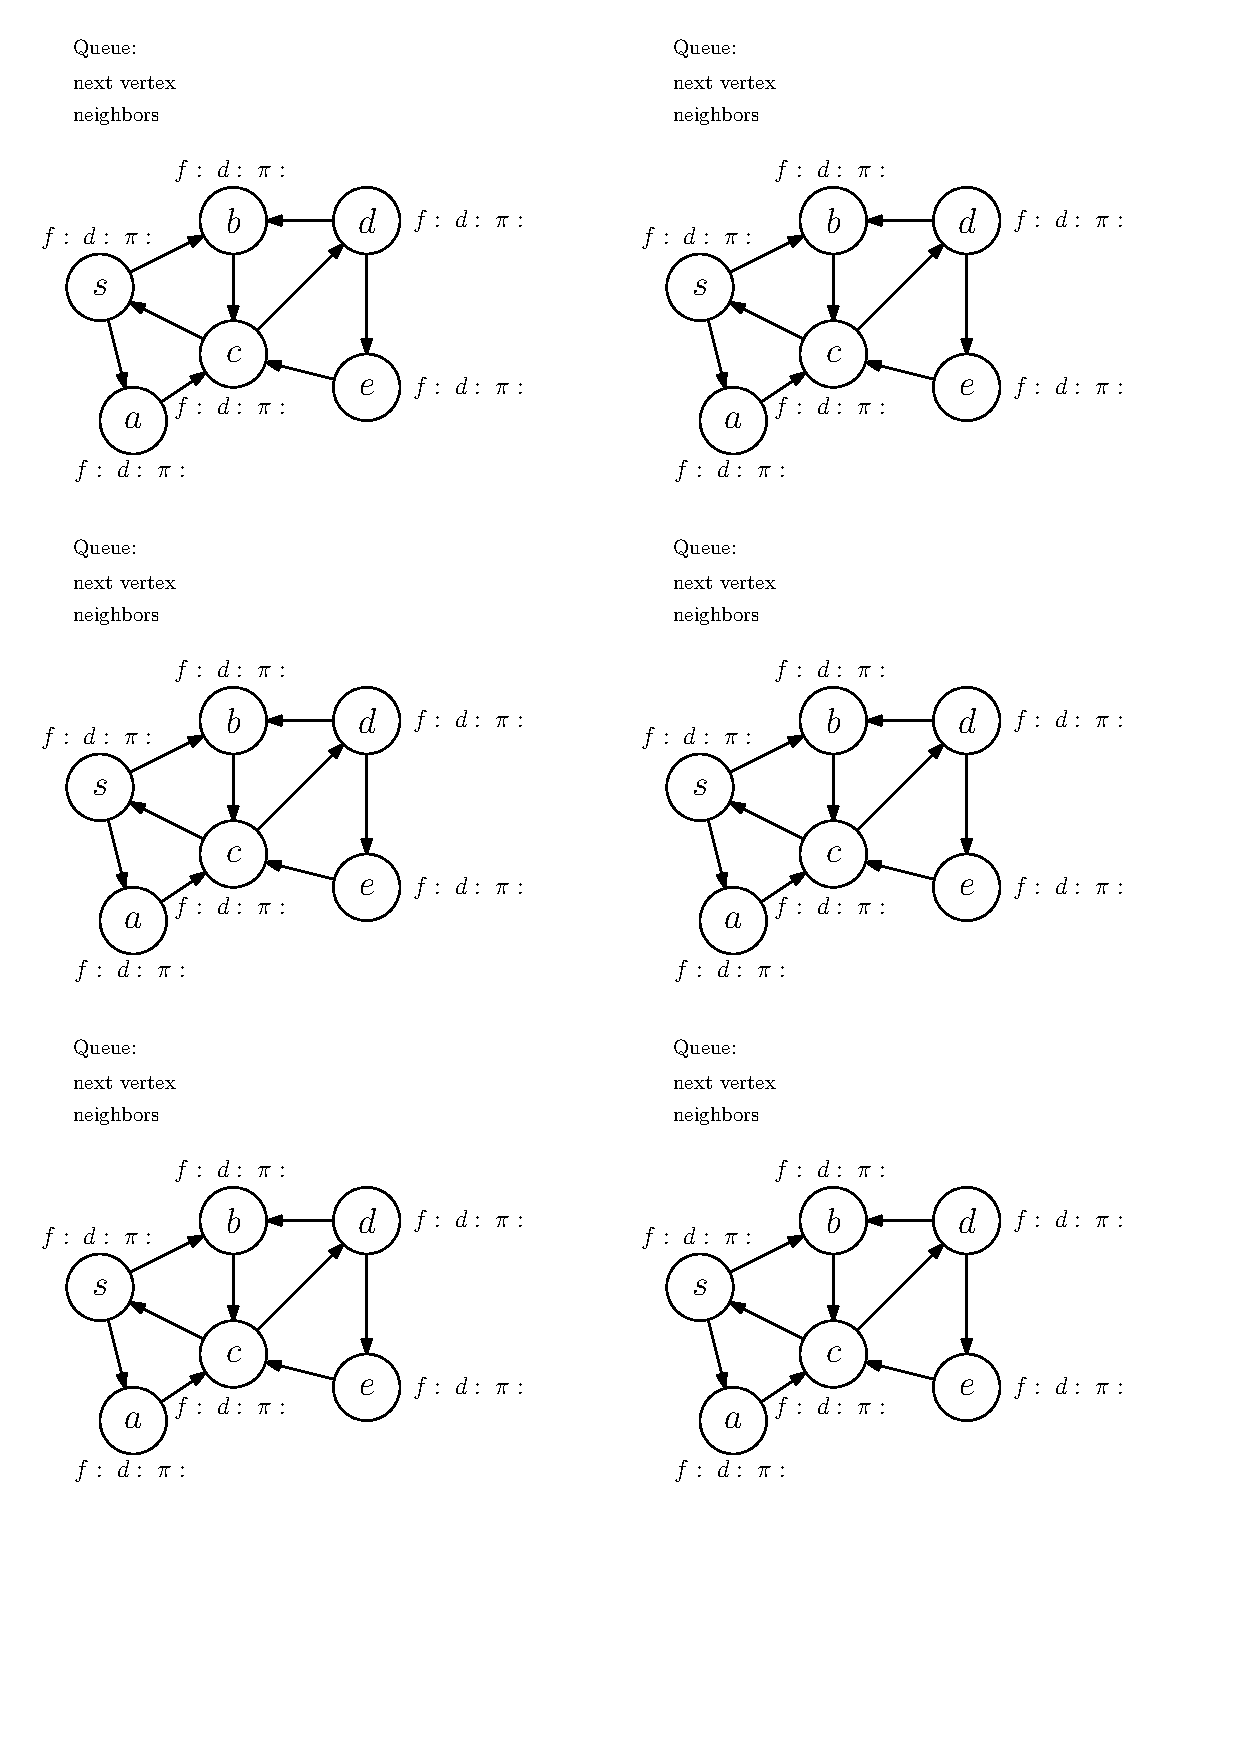
\includegraphics[scale=0.8]{bfs}
\end{center}
\end{description}
\end{document}
